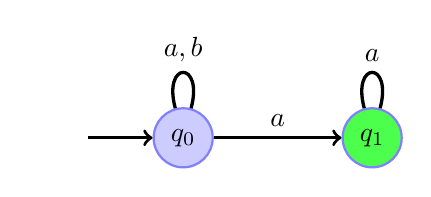
\begin{tikzpicture}[scale=0.8]
	\node 	(q)		at	(-2,0) 	[circle, thick,minimum size=.75cm]{};

	\node 	(q0)		at	(0,0) 	[circle, thick, draw=blue!50,fill=blue!20,inner sep=0pt,minimum size=.75cm]{$q_0$};


	\node 	(q1)		at	(3,0) 	[circle, thick, draw=blue!50,fill=green!70,inner sep=0pt,minimum size=.75cm]{$q_1$};

	\draw[loop above,very thick] (q0) to 	node[auto]{$a,b$} 		(q0);
	\draw[loop above,very thick] (q1) to 	node[auto]{$a$} 		(q1);
	\draw[->,very thick] (q0) to 	node[auto]{$a$} 		(q1);
	\draw[->,very thick] (q) to 	node[auto]{} 		(q0);

\end{tikzpicture}
